\begin{post}
	\postdata{The Best College Day™}{2011}{11}{8}{1}{57}{41}
	\begin{content}
\textit{Writing a blog is sometimes quite hard. Yesterday, this post had almost 1100 words. Then I realized it is boring and too "iterative" (I did this and then that and after that something else), and I deleted it, because I promised to myself that I won't write in this "diary" style. You are not interested in my daily life, right...so instead of writing a lot of stuff about The Best College Day™, I will try to keep it short so you have enough time to do your own things. So watch a movie afterwards. Or walk your dog. Or something...}

There are few things that you need to have the best day. \textbf{The weather} has to be nice. There has to be some \textbf{activity that you like}. There have to be your \textbf{friends}. There has to be some good \textbf{food}. There have to be \textbf{drinks}. There has to be\textbf{ the right mood}. Combine all that, and you have the best recipe for an awesome day. Just do not overcook it, please.

Firstly, the weather. On Thursday, November 3rd, the weather was amazing. The sun was shining, the sky was blue, the birds were singing. I was walking around just in a t-shirt, because it was so warm. So weather — \textcolor{Chameleon}{check!}

Favorite activities. Hmm, that might be more difficult. I like a lot of things — bikes, music, bass, golf, running, you name it. But I don't have my bass or my bike here, there are no good concerts around and running on a treadmill is not that exciting either. So what is left? Yep, golf. As a part of the KAIST Autumn Festival, there was a screen golf competition, in which I participated. I sucked, honestly, partly because my golf skills were too big to bring them to Holland and then to Seoul, but I had an awesome time, because I could play a round just for fun — no ambitions, no scorecards, no pressure. \textcolor{Chameleon}{Check!}

Friends. This one is easy. I really like our exchange group here, as well as other full time students. And since no student ever refuses free things, everybody was participating. \textcolor{Chameleon}{Check!}

\begin{wrapfigure}{R}{0.5\textwidth}
\centering\fbox{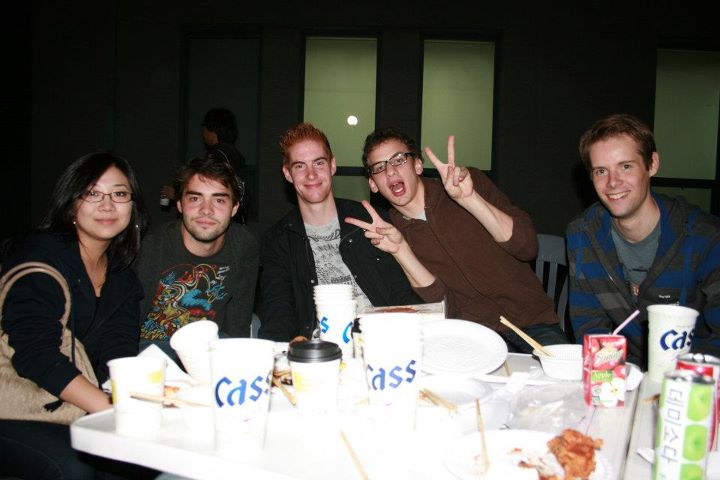
\includegraphics[width=0.5\textwidth]{photos/11/08/group.jpg}}\vspace{-32pt}
\end{wrapfigure}


And that brings me to the food and drinks issue. For the festival, KAIST provided food and drinks for everybody. Chicken wings, kimbap, pancakes, sweets, sours, everything was there. And tap beer as well. And, of course, everything for free. If you consider that the "food court" was located outside, in the middle of the campus, under the sun and the blue sky...so \textcolor{Chameleon}{check} as well!

And now to the difficult part, the mood. You can't influence that. But the state of the world can. It's hard to have a bad mood when you are having a good time. \textcolor{Chameleon}{Check!}

So, to sum it up. Last Thursday was perfect. I think I really had The Best College Day™ so far. Apart from all the things mentioned above, I have also participated in a beer drinking competition, saw a K-POP performance, had a BigMac menu delivered to the campus, went dancing, sang Backstreet Boys and ended up with orange ribbons tied to my glasses. And I won a little mechanical snail in a raffle. Seriously, that sounds like fun, right...

And \textcolor{Chameleon}{check}!
	\end{content}
\end{post}
